\section{Rayleigh-Streuung}
Weil diese Bilder so schön sind, hier noch ein weiteres.
\xfigure{htbp}{width=\textwidth}{Sunsetboot.png}{}{Sonnenuntergang mit Polizeitboot auf dem Weg von der Uni zum Bahnhof}

\section{Code-Anhang}
Die \verb|.jpynb| Datei, mit vollständigem Code (an manchen Stellen ist etwas in der pdf-Datei abgeschnitten), findet sich auch in der \href{https://heibox.uni-heidelberg.de/d/2efd363da5f84ceea685/}{Heibox}.
Leider wird der Klick Progress in der \verb|.html| Datei nicht gespeichert, deswegen sieht man leider nicht alle Bilder mit der Halbwertsbreite, ich habe eines beispielsweise in eine Markdownzelle reinkopiert.
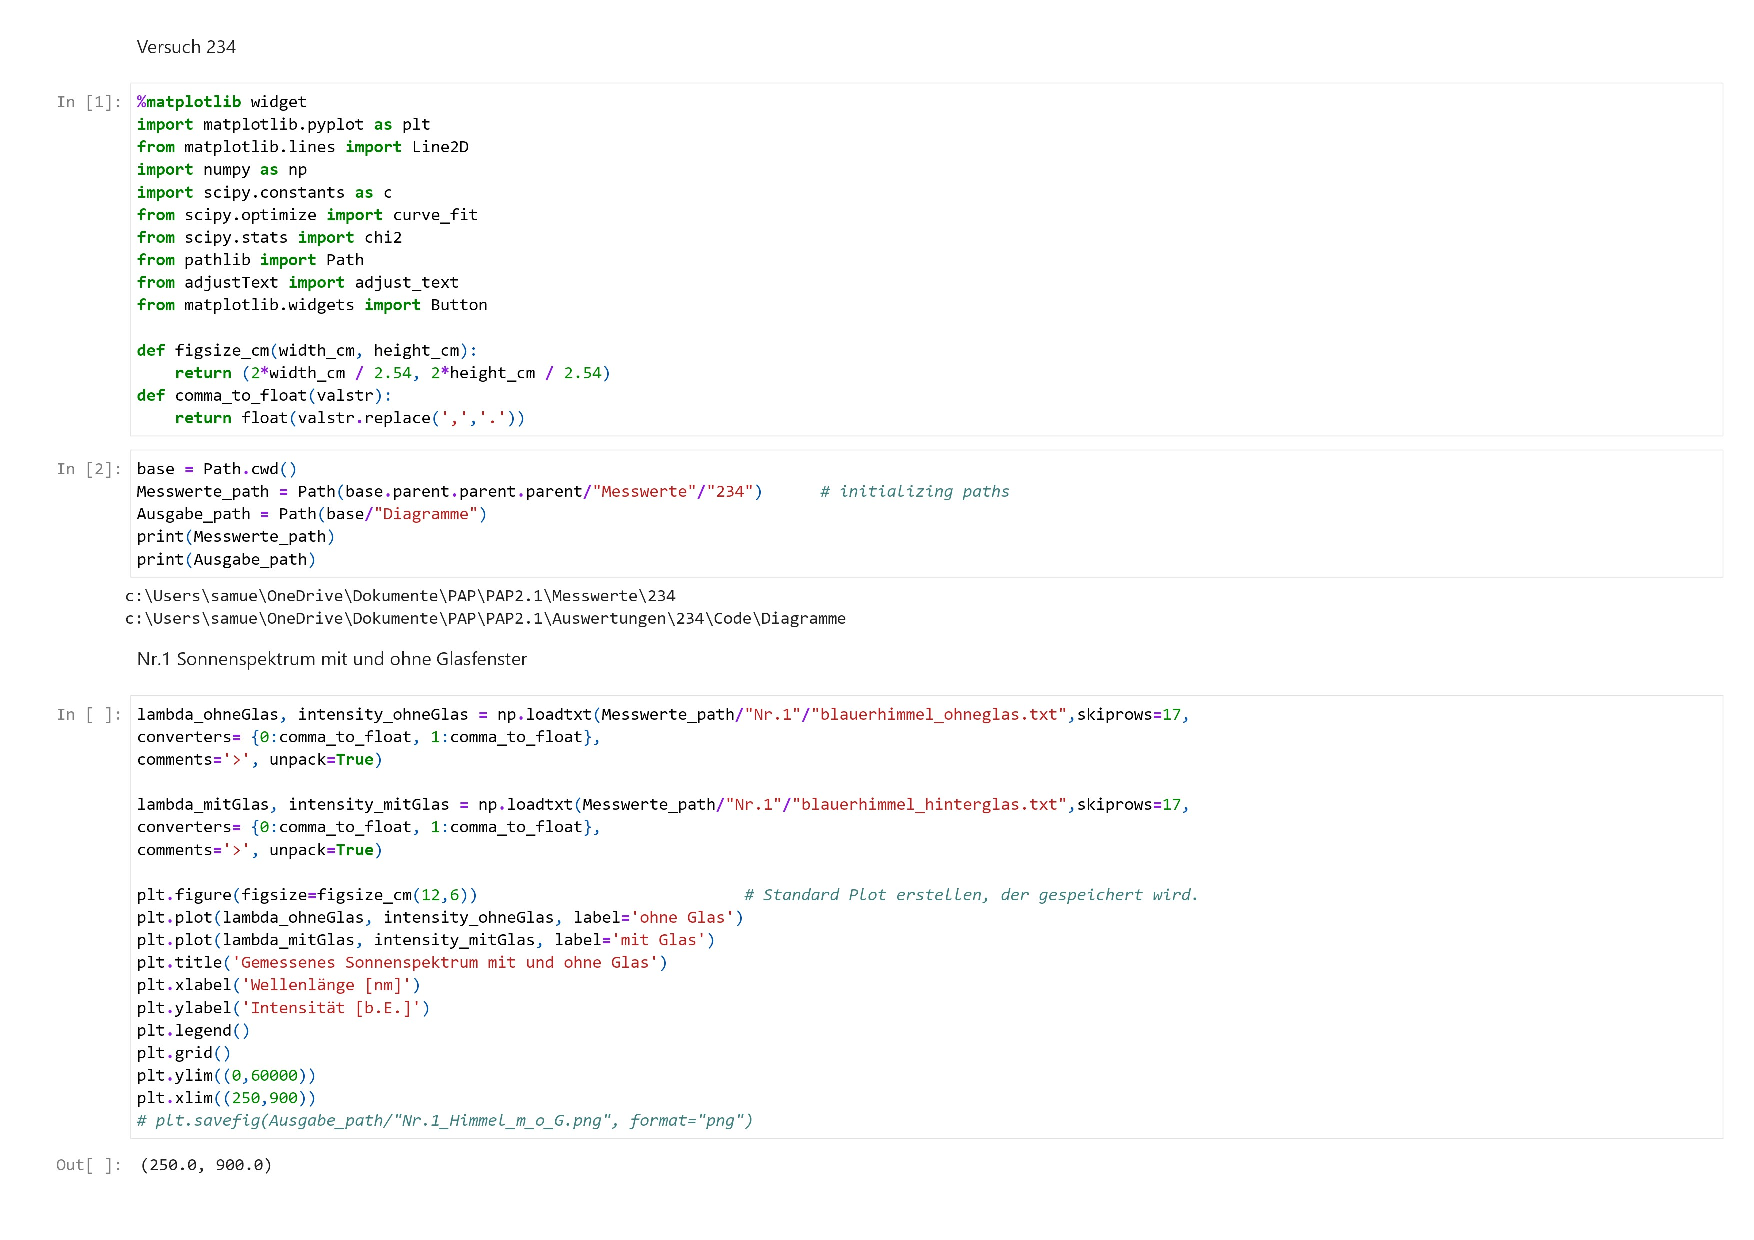
\includepdf[landscape=true,pages=-]{../Code/234/234.pdf}
